\section{Kapcsolási rajz}

\subsection{ESP8266 programozó}
Az mikrokontrollernek három különböző boot módja van. Az adott mód kiválasztása 3 db láb megfelelő állapotba állításával lehetséges. A panelon egy 6 pines csatlakozón keresztül lehet UART segítségével programozni. A programozó ezenkívűl egy tranzisztor segítségével tudja automatikusan a kód feltöltése során programozható állapotba állítani az eszközt. A kapcsolási rajzon tovább látható, hogy bizonyos lábakat fel, illetve lekell húzni a megfelelő működéshez. Későbbiekben a használható perifére kombinációknal ezeket figyelembe kell venni, mert ezzel is szűkül az elérhető lábak felhasználhatósága.

\begin{figure}[!ht]
    \centering
    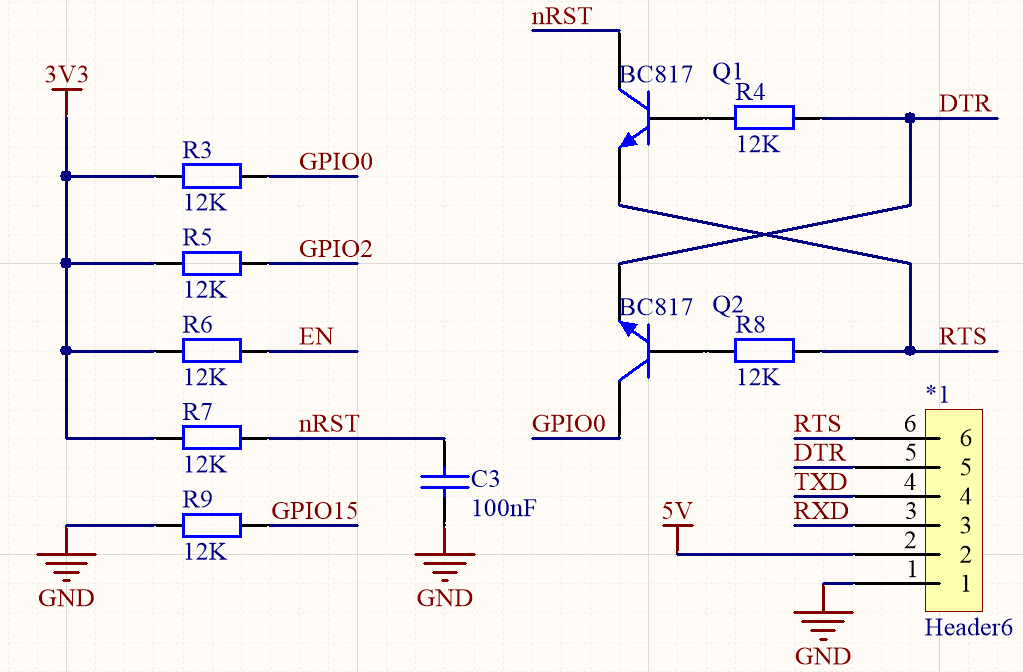
\includegraphics[width=130mm, keepaspectratio]{figures/programmer.png}
    \caption{ESP8266 programozó bekötése}
    \label{fig:TeXstudio}
\end{figure}

\begin{table}[ht]
	\footnotesize
	\centering
	\begin{tabular}{ | c | c | c | c | c |}
		\toprule
		GPIO15 & GPIO0 & GPIO2 & mód & leírás \\
		\midrule
        Alacsony & Alacsony & Magas & UART & Kód letöltése UART-ról \\
        \hline
        Alacsony & Magas & Magas & Flash & Boot SPI Flash-ből \\
        \hline
		Magas & x  & x & SDIO & Boot SD kártyáról \\
		\bottomrule
	\end{tabular}
	\caption{ESP8266 boot módok}
	\label{tab:TabularExample}
\end{table}
Az ESP lehetőséget biztosít, hogy vezetéknélkül is lehessen frissíteni a firmware-t OTA ( Over The Air) használatával. Ebben az esetben szükséges egy webszervert is használni, illetve figyelembe kell venni a különböző biztonsági kockázatokat.

% alap lábbekötések
% A modul programozása egy 6 pines csatlakozón (Rx,Tx,RTS,DTS,5V,GND) keresztül UART segítségével történik.
\subsection{FET meghajtó áramkörök}
A mikrokontroller lábai maximálisan 12 mA-al terhelhetőek, ezért szükséges különböző meghajtó áramkörök használata. A modulon helyett kapott 2 db P-csatornás, 4 db N-csatornás MOSFET kimeneti meghajtó, illetve elérhető 2db N csatornás MOSFET-el megvalósított bemenet is.

Az N csatornás kimenetek esetében lehetőség van kiválasztani a kapcsolt feszültséget egy forrszem segítségével. Ez lehet 5V vagy a bemeneti tápfeszültség, ami maximálisan 12V. Továbbá külön beállítható ezeknél a kimeneteknél az alapértelmezett állapot a megfelelő fel vagy lehúzó ellenállás beforrasztásával. Az védelem érdekeben ezenkívúl belett tervezve egy dióda induktív terhelés esetére.

\begin{figure}[!ht]
    \centering
    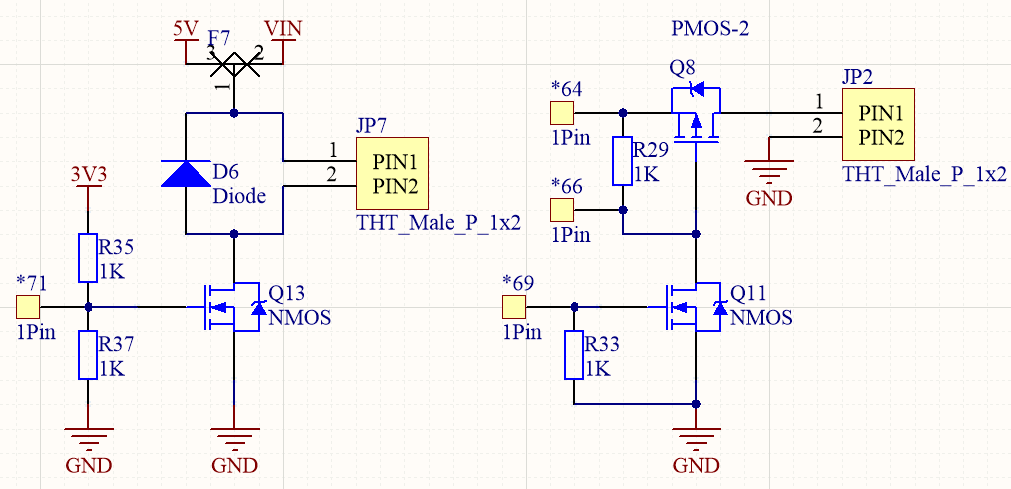
\includegraphics[width=140mm, keepaspectratio]{figures/n_p_driver.png}
    \caption{N és P csatornás MOSFET meghajtók}
    \label{fig:TeXstudio}
\end{figure}

\begin{figure}[!ht]
    \centering
    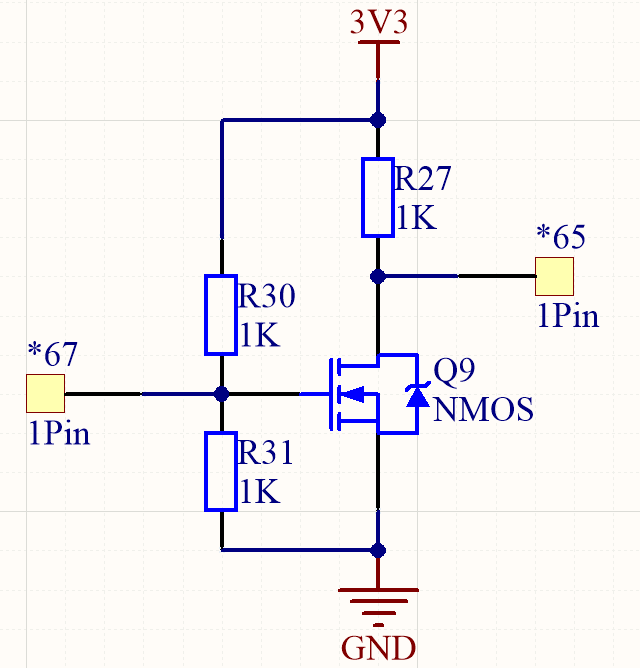
\includegraphics[width=55mm, keepaspectratio]{figures/n_input.png}
    \caption{N csatornás MOSFET bemenet}
    \label{fig:TeXstudio}
\end{figure}

\subsection{Optokapu}
2 db optokapunak lett hely kialakítva a panelon, amik például P-csatornás MOSFET meghajtóval kombinálva izolált vezérlést tesz lehetőve.

\begin{figure}[!ht]
    \centering
    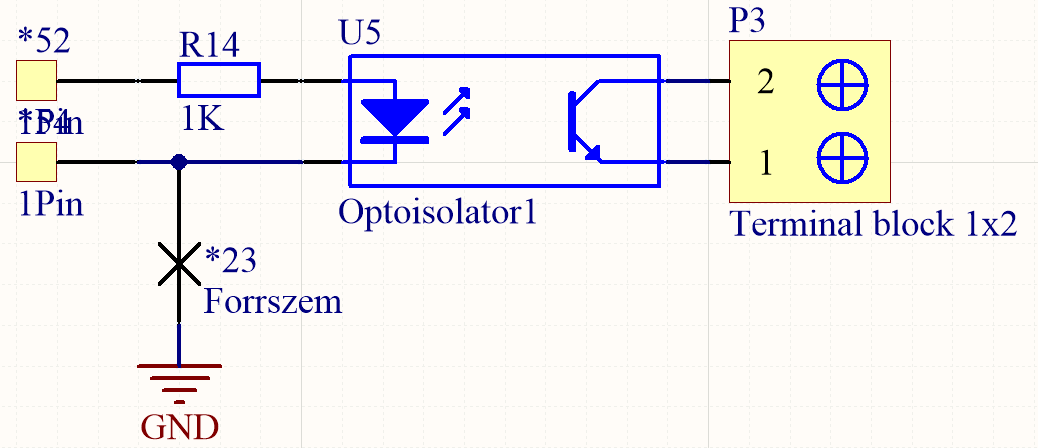
\includegraphics[width=100mm, keepaspectratio]{figures/opto.png}
    \caption{Optokapu}
    \label{fig:TeXstudio}
\end{figure}


\subsection{I2C}
Az ESP8266-nak alapértelmezetten egy I2C interfésze van, ami szoftveresen van megvalósítva. Erre az interfészre kapcsolódik a panelon elhelyezkedő kijelző, hőmérséklet szenzor, illetve shift regiszter. Lehetőség van ezenkívűl további perifériák egyszerű csatlakoztatására is, mivel helyet kapott külön kivezetés tüskesorra is.

A panelon elhelyezett hőmérséklet szenzor egy LM75-ös digitális hőmérő, aminek SOP8 tokozása van. Számos más hőmérséklet, illetve párataratalom mérő szenzor is használható a megegyező lábkiosztásnak köszönhetően.
\begin{figure}[!ht]
    \centering
    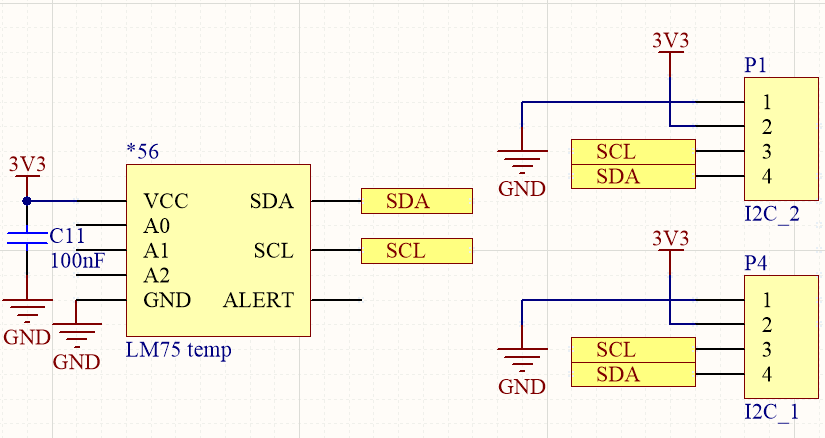
\includegraphics[width=130mm, keepaspectratio]{figures/i2c_devices.png}
    \caption{Hőmérséklet szenzor, illetve I2C kivezetések}
    \label{fig:TeXstudio}
\end{figure}


\subsection{Enkóder}
Lehetőség van egy kapcsolóval egybeépített enkóder bekötésére a panelon. Ennek a fő szerepe a kijelző által biztosított menürendszerben való navigálás. A kijelző hiánya esetében is több funkció rendelhető hozzá például a különböző kimenetek szabályzása. A beépített nyomógomb egy interrupt segítségével például beállítható, hogy visszakapcsoljon alvás üzemmódból a mikrokontroller.


\subsection{Shift regiszterek}
A mikrokontrollernek mivel viszonylag kevés szabad GPIO lába áll rendelkezésre, ezért lehetőség van a különböző shift regiszterek használatával növelni az elérhető bemenetek és kimenetek számát, ha az alkalmazáshoz szükséges. A panelon 2db 8 bit-es SPI interfészel, illetve egy 16 bit-es I2C-vel rendelkező shift regiszter helyezhető el. A 8 bitesek egyike párhuzamos bemeneteket alakít sorossá. A másik pedig soros bemenetet alakít át párhuzamos kimenetekké. 
\begin{figure}[!ht]
    \centering
    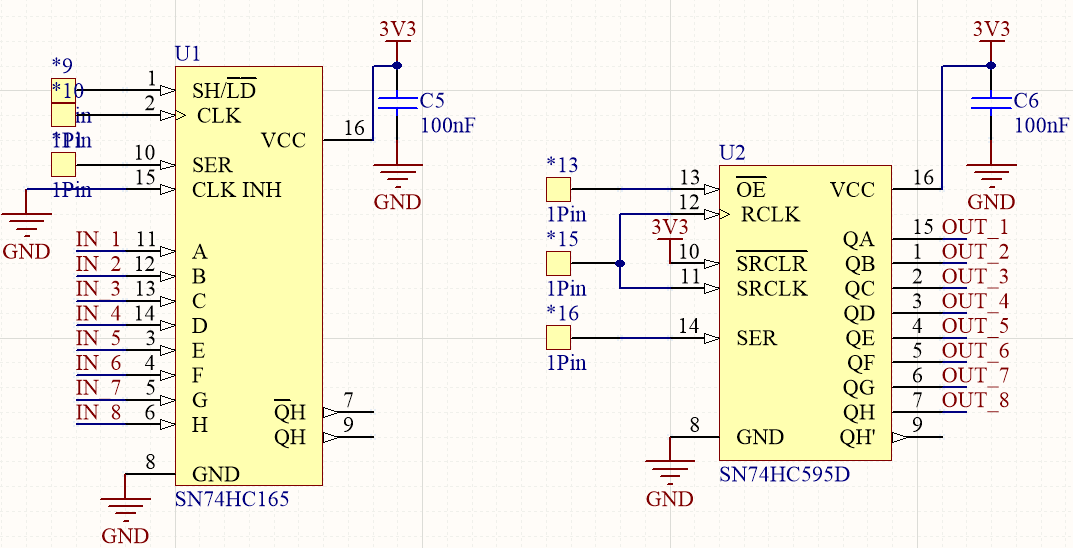
\includegraphics[width=140mm, keepaspectratio]{figures/8bit_shift_registers.png}
    \caption{8bites shift regiszterek kapcsolási rajza}
    \label{fig:TeXstudio}
\end{figure}
A 16 bites shift regiszteren külön konfigurálható, hogy milyen állapotban legyenek a lábai. Egy plusz funkció, hogy interrupt rendelhető bármelyik bemeneti módban lévő lábhoz. A felhasznált terület csökkentése érdekében, illetve mivel nem minden alkalmazáshoz szükséges plusz bemenet vagy kimenet, ezért a 16bites és a 8bites IC-k ki és bemenetei ugyanazokra a lábakra vannak kivezetve.
\begin{figure}[!ht]
    \centering
    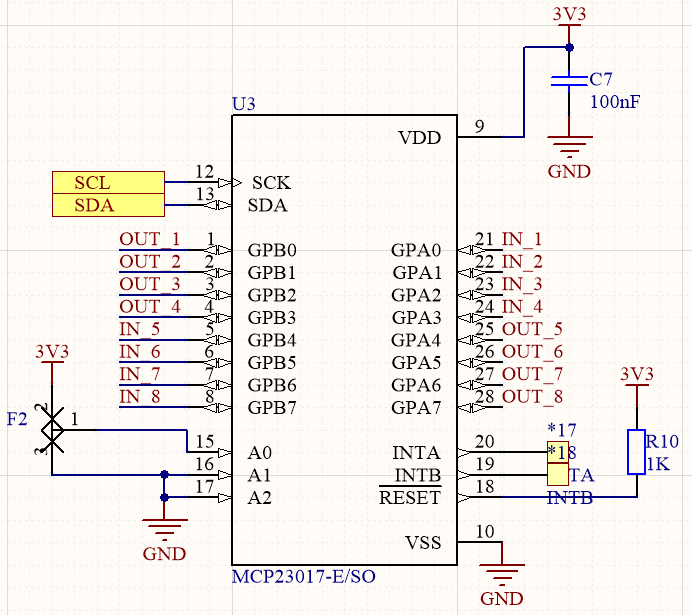
\includegraphics[width=95mm, keepaspectratio]{figures/16bit_shift_register.png}
    \caption{16bites shift regiszter kapcsolási rajza}
    \label{fig:TeXstudio}
\end{figure}


\subsection{Infra adó/vevő}
Számos otthoni eszköz használ különböző infrás megoldásokat főleg a távoli vezérléshez. Ezeknek az eszközöknek az illesztése érdekeben a panelen helyett kapott egy infra adó/vevő, amit a mikrokontroller erre szánt lábaira bekötve létrejöhet a kommunikáció. Lehetőség van ezáltal a már meglévő távirányítókkal a modul irányítása is, így például elhagyható az enkóder használata.
A infra led meghajtása egy N csatornás MOSFET-el történik, mivel nagyobb áram szükséges a LED meghajtásához, mint a mikorokontroller lába által biztosított 12 mA.
\begin{figure}[!ht]
    \centering
    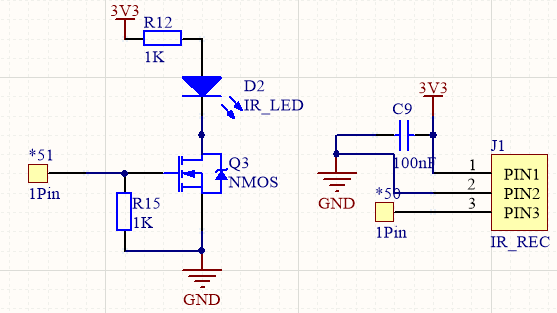
\includegraphics[width=130mm, keepaspectratio]{figures/infra.png}
    \caption{Infra adó/vevő}
    \label{fig:TeXstudio}
\end{figure}


\subsection{Kijelzők, LED-ek}
Opcionálisan elhelyezhető a panelon egy I2C interfésszel rendelkező 128x64-es felbontású OLED kijelző. A kijelzőn könnyen megjelenhítőek az eszközhoz kapcsolt különböző szenzorok értékei minimális kód hozzáadásával. Megjeleníthetők továbbá alapvető információk pl. hálozat állapota, GPIO pinek állapota is, amik segítségül szolgálhatnak az adott alkalmazás fejlesztésénél.
\begin{figure}[!ht]
    \centering
    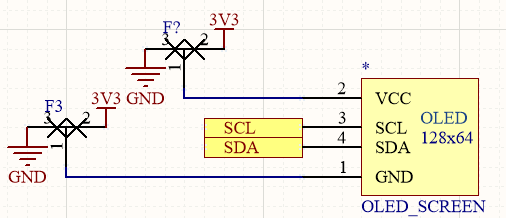
\includegraphics[width=120mm, keepaspectratio]{figures/display.png}
    \caption{OLED kijelző bekötése}
    \label{fig:TeXstudio}
\end{figure}

Elérhető továbbá egy normál, illetve egy RGB led, amiket szintén sokféle képpen lehet felhasználni. A kijelző elhagyása esetén lehet állapot jelzőnek használni. A panelre nem került külön led a tápfeszültség meglétének jelzésére, de a ledhez tartozó mindkét forrszem beforrasztásával ez is megoldható. Az RGB led vezérléséhez 5 V-os jelszint szükséges. A kapcsoláson jól látható, hogy egy "és" kaput használva történik a jelszint átalakítás. Az "és" kapu a bemenetére kötött 3,3 V-ot már logikai 1-esnek érzékeli, illetve a bemenetei összevannak kötve, ezért a kimenetet éppen a bejövő jelnek megfelelően kapcsolja.
\begin{figure}[!ht]
    \centering
    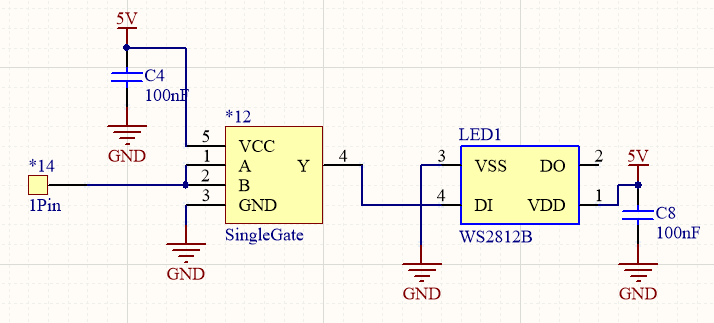
\includegraphics[width=150mm, keepaspectratio]{figures/rgb_led.png}
    \caption{RGB Led}
    \label{fig:TeXstudio}
\end{figure}
Egyszerű számok, illetve időpontok kijelzésére elegendő lehet csak néhány 7 szegmenses kijelző. Ezt figyelembe véve ki lett alakítva egy csatlakozástatási pont, ahova egy ilyen kijelzőket tartalmazó modul köthető be.
\begin{figure}[!ht]
    \centering
    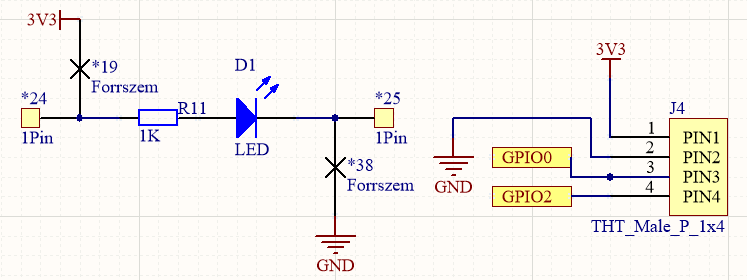
\includegraphics[width=150mm, keepaspectratio]{figures/led_connector.png}
    \caption{Led, 7 szegmenses kijelző csatlakoztatási pont}
    \label{fig:TeXstudio}
\end{figure}



\subsection{ADC}
Az ESP8266 mikrokontrollernek csak egy darab lába képes analóg bemenetet olvasni. Az átalakítást egy 10 bites ADC végzi, aminek a bemeneti tartománya 0-10V-ig terjed. A bemenet átskálázását egy feszültségosztóval állítható be. Akkumlátoros tápellátás esetén például használható a bemeneti tápfeszültség mérésére.

\subsection{Tápellátás}
A megvalósított eszköz tápellátására több lehetőség is biztosított. Egyrész található rajta egy szabványos tápcsatlakozó, amire DC 6.5V - 12V feszültség csatlakoztatható. A másik lehetőség egy micro USB-n keresztül 5V-os bemenet, illetve a programozón keresztül is lehetséges az áramkör táplálása. A bejövő feszültséget két darab lineáris feszültségszabályzó alakítja át. Az első 5V-ra majd ennek a kimenete rá van kötve egy 3,3V-ot előállítóra. A stabil feszültségek biztosítása érdekében szűrő kondenzátorok kerültek az IC-k ki és bemeneteire is. A további kiegészítő áramkörök egyszerű tápellátása érdekében a különböző tápfeszültségek több ponton is kilettek vezetve a NYÁK-on.

\begin{figure}[!ht]
    \centering
    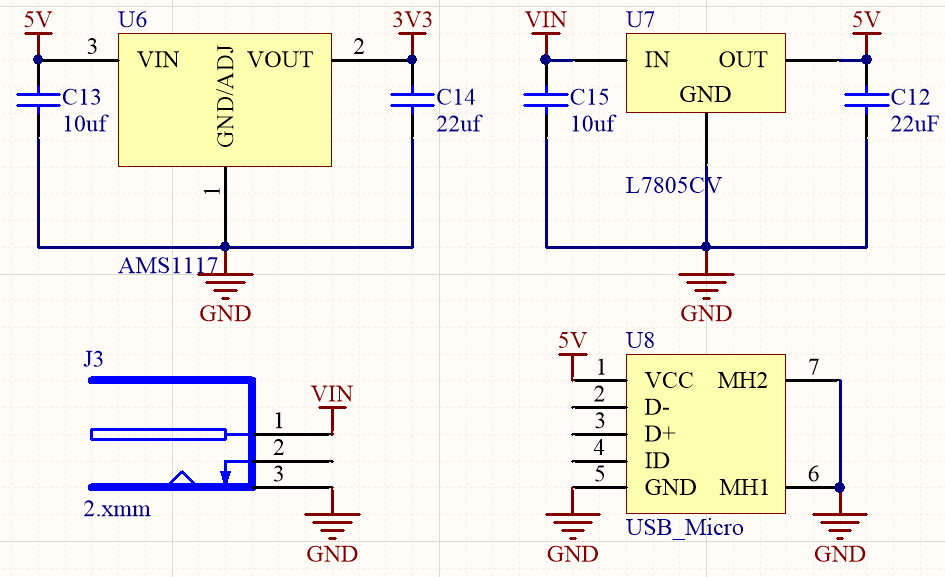
\includegraphics[width=130mm, keepaspectratio]{figures/power.png}
    \caption{Tápellátás}
    \label{fig:TeXstudio}
\end{figure}


